236. \begin{figure}[ht!]
\center{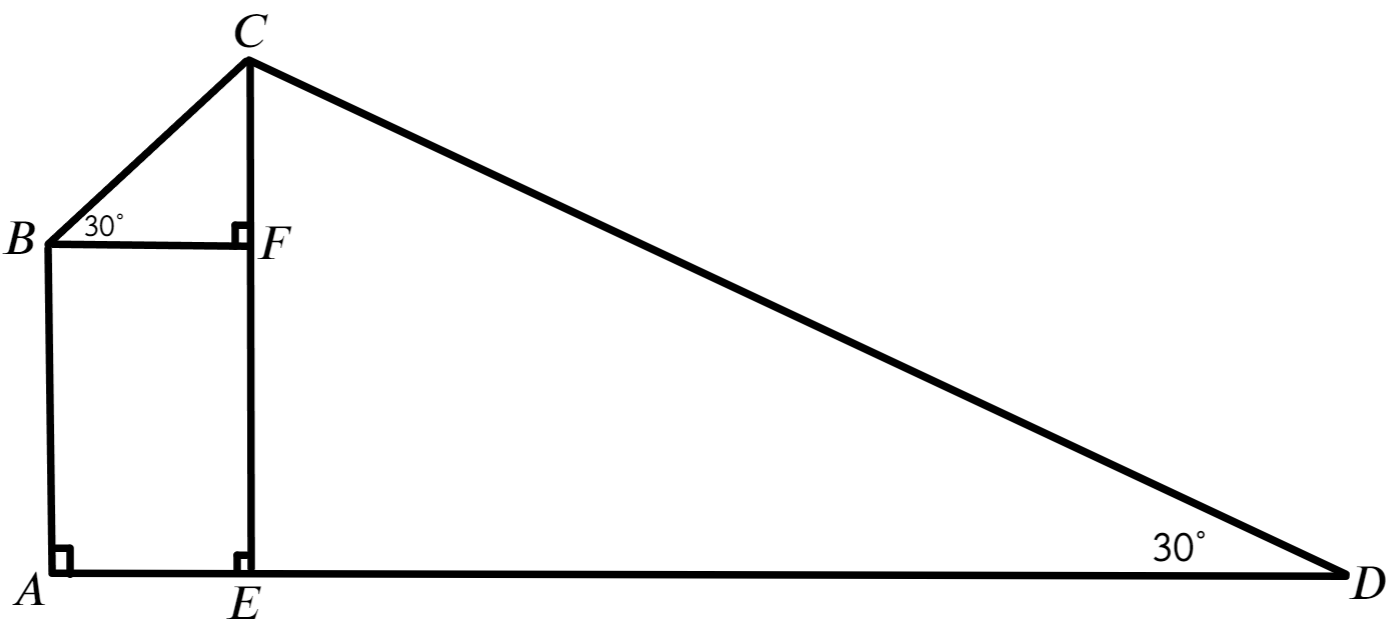
\includegraphics[scale=0.35]{g8-235.png}}
\end{figure}\\
Опустим из точки $C$ на сторону $AD$ перпендикуляр $CE,$ а из точки $B$ на $CE$ --- перпендикуляр $BF.$ Тогда $ABFE$ --- прямоугольник и $FE=AB=3,$ а $\angle CBF=  120^\circ-90^\circ=30^\circ.$ По теореме о катете, лежащем напротив угла в $30^\circ,$ имеем равенства $CF=\cfrac{1}{2}BC=1,\ CD=2CE=2(CF+FE)=2(1+3)=8.$\\
